\section{Analysis of the Measurements}
\subsection{Absorption Spectrum}
First we analyse the measurement of the absorption spectrum with the CCD-Spectrometer. Here only the measurement over $30$ scans \verb|abs30.csv| is used. First the whole spectrum was plotted in figure \ref{figAS1}.
\begin{figure}[ht]
	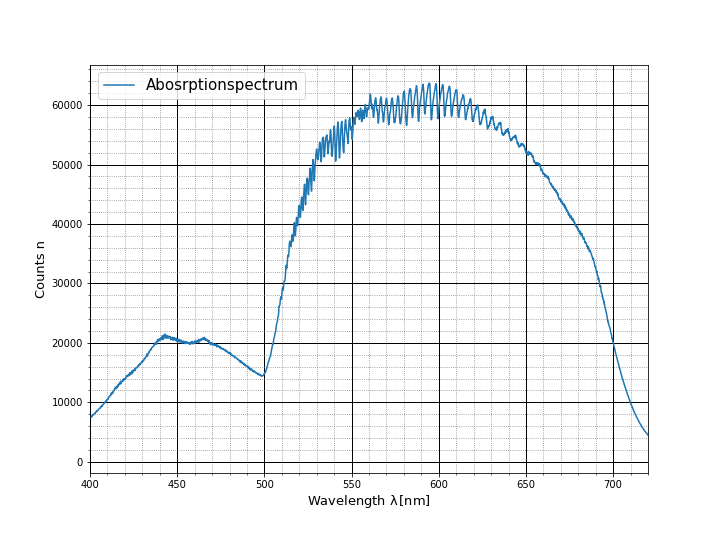
\includegraphics[scale=0.5]{Bild/AS_1.png}
	\centering
	\caption[Complete Absorption Spectrum]{\small Here is the complete absorption spectrum from $400$nm to $720$\,nm. Measured with the CCD-Spectrometer.}
	\label{figAS1}
\end{figure}
The spectrum goes from $400\,$nm to $720$\,nm. In the spectrum we are interested in the vibration transitions, which can be seen as dips in the spectrum. In the manual\cite{Anleitung} the transition $\nu''=0\rightarrow \nu'=25$ at a wavelength of $545.8\,$nm is given as reference. That's why the area of $505\,$nm to $570\,$nm was picked to find further transitions, which can be seen in figure \ref{figAS2}.\par
To find the peaks the spectrum was inverted and the Python package \verb|PeakUtils| was used to find the peaks. In figure \ref{figAS2} the furthest to the right marked peak is the reference peak of the $\nu''=0\rightarrow \nu'=25$ transition. Further to the right are also peaks visible, but they are starting to mix with other peaks which indicates that here another transition superimposes on the first one. That's the reason these peaks were left out. Overall the transitions from $\nu''=0\rightarrow \nu'=25$ to $\nu''=0\rightarrow \nu'=47$ were likely found. The positions are noted inside the table \ref{tabAS1}. Here an error of $0.5\,$nm was estimated since \verb|PeakUtils|\cite{Peak} doesn't give errors on the positions. \par
\begin{figure}[ht]
	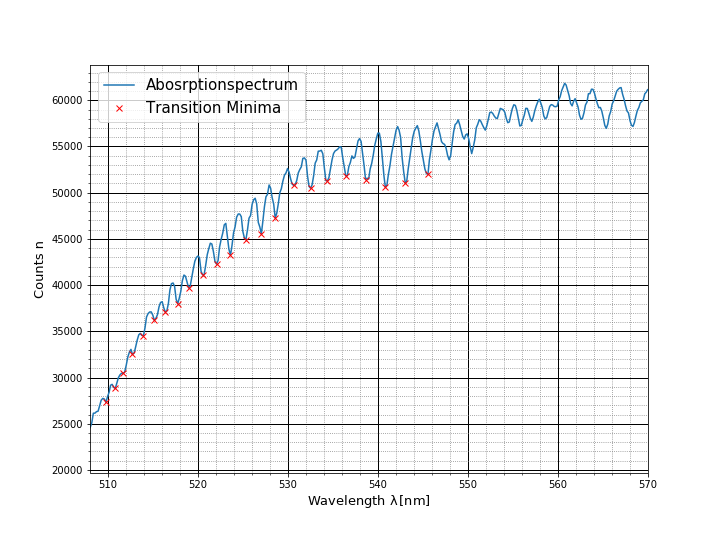
\includegraphics[scale=0.5]{Bild/AS_2}
	\centering
	\caption[Absorption Spectrum with Transitions]{\small Absorption spectrum from $509\,$nm to $570\,$nm. In red are the absorption minima of the different vibration transitions. Starting left with the $\nu''=0\rightarrow \nu'=47$ transition till at the right side we got the $\nu''=0\rightarrow \nu'=25$ reference transition.}
	\label{figAS2}
\end{figure}
\FloatBarrier
\subsubsection{Calculating $\omega_ex_e$ and $\omega_e$}
With these positions a Birge-Sponer-Plot can be created to calculate the constants $\omega_e$ and $\omega_ex_e$. For this the wavelength were used to calculate the energy of the absorbed photons. For this Equation \ref{eqEnergie} was used. The error was like all calculated with the python package \verb|uncertainties|\cite{uncertainties} which itself uses Gaussian propagation of uncertainties.
\begin{equation}
	G(\nu'')=\frac{1}{\lambda}, \qquad \sigma_G=\frac{\sigma_\lambda}{\lambda^2}
	\label{eqEnergie}
\end{equation}
Since the energy difference between two adjacent transitions $\Delta G(\nu+\frac{1}{2})$ is needed for the plot these were calculated next. 
\begin{equation}
	\Delta G(\nu+\frac{1}{2}) = G(\nu+1)-G(\nu) 
\end{equation}
The error is calculated with the following equation:
\begin{equation}
	\sigma_{\Delta G} = \sqrt{\sigma_{G(\nu+1)}^2+\sigma_{G(\nu)}^2}
\end{equation}
These are now plotted against $\nu+\frac{1}{2}$ in figure \ref{figAS3}. By fitting a line of the form $y=mx+b$ to these values the constants can be calculated using equation \ref{eq1} and \ref{eq2}.\par
\begin{equation}
	\omega_ex_e = -\frac{m}{2}, \qquad \sigma_{\omega_ex_e}=-\frac{\sigma_m}{2}
	\label{eq1}
\end{equation}
\begin{equation}
	\omega_e=b+\omega_ex_e, \qquad \sigma_{\omega_e}=\sqrt{\sigma_b^2+\sigma_{\omega_ex_e}^2}
	\label{eq2}
\end{equation}
The fit was realised using the python package \verb|curve_fit|\cite{SciPy_Opti} which also considers the errors in the $y$ direction. With that the following parameters were calculated:
\begin{equation*}
	m = (-2.09\pm 0.13)\,\text{cm}^{-1} \qquad \text{and} \qquad b = (133\pm 4)\,\text{cm}^{-1}
\end{equation*}
For the two constants $\omega_ex_e$ and $\omega_e$ we get:
\begin{equation*}
	\omega_e = (135\pm 5)\,\text{cm}^{-1}
\end{equation*}
\begin{equation*}
\omega_ex_e = (1.04\pm 0.07)\,\text{cm}^{-1}
\end{equation*}
\begin{figure}[ht]
	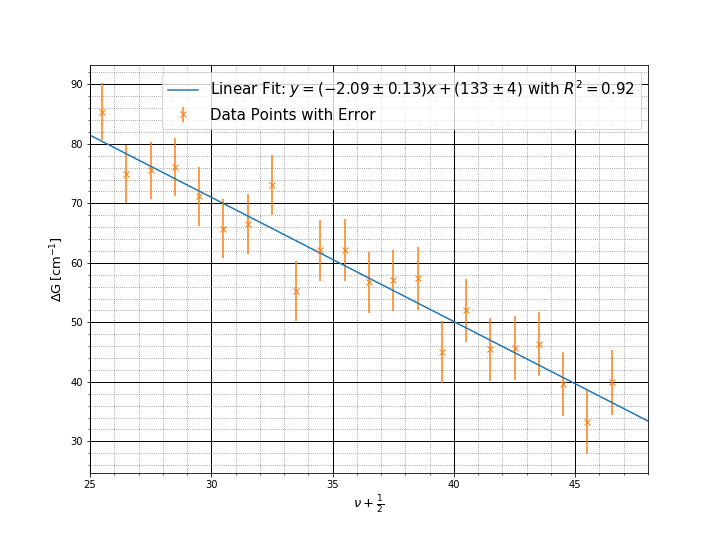
\includegraphics[scale=0.5]{Bild/AS_3}
	\centering
	\caption[Birge-Sponer-Plot with Linear Fit]{\small Birge-Sponer-Plot with Linear Fit in blue. In orange the data points of the values $\Delta G$ which can be found in table \ref{tabAS1} with errors.}
	\label{figAS3}
\end{figure}
\subsubsection{Dissociation Energy}
We now calculate the dissociation energy $D_{e_1}$ in two different ways. First we use the equation \ref{eqDis} we got from the Morse Potential using both of the computed constants. The second way is using the sum in equation \ref{D0} to get the energy $D_0$. By adding $G(\mu=0)$ to this the dissociation energy $D_{e_2}$ can be calculated.\par
For the first method the error is calculated using the following equation:
\begin{equation}
	\sigma_{D_e}=\sqrt{\left(\frac{\sigma_{\omega_e}\omega_e}{2\omega_ex_e}\right)^2+\left(\frac{\sigma_{\omega_ex_e}\omega_e^2}{4(\omega_ex_e)^2}\right)^2}
\end{equation}
With that we get for $D_{e_1}$:\par
\begin{equation*}
	D_{e_1}=(4300\pm 400)\,\text{cm}^{-1}
\end{equation*}
Now we use the second method to calculate $D_0$. The error here is calculated with equation \ref{eqsumerror}:
\begin{equation}
	\sigma_{D_0}=\sqrt{\left(\sum_{\nu=0}^{\nu_{diss}}\sigma_{\Delta G (\nu+\frac{1}{2})}^2\right)}
	\label{eqsumerror}
\end{equation}
$G(0)$ is calculated using equation \ref{eqBSP} till the quadratic term. We get as equation to calculate $G(0)$:
\begin{equation}
	G(0)=\frac{\omega_e}{2}-\frac{\omega_ex_e}{4}, \qquad \sigma_{G(0)}=\sqrt{\left(\frac{\sigma_{\omega_e}}{2}\right)^2+\left(\frac{\sigma_{\omega_ex_e}}{4}\right)^2}
\end{equation}
The calculated values are:
\begin{equation*}
	D_0=(4280\pm 60)\,\text{cm}^{-1}
\end{equation*}
\begin{equation*}
G(0)=(67.1\pm 2.4)\,\text{cm}^{-1}
\end{equation*}
Adding these two together the error is:
\begin{equation}
	\sigma_{D_{e_1}}=\sqrt{\sigma_{G(0)}^2+\sigma_{D_0}^2}
\end{equation}
The value for $D_{e_2}$ is with that:
\begin{equation*}
	D_{e_2}=(4340\pm 60)\,\text{cm}^{-1}
\end{equation*}
\subsubsection{Excitation Energy $T_e$ and Dissociation Energy $E_{diss}$}
The energy $E_{diss}$ is the energy between first vibration state of the electronic ground state and the dissociation state of the the exited electronic state. This energy can be found by looking at the lowest point of the spectrum where no vibration dips can be found. The estimated position can be seen in figure \ref{figAS4}.
Since this point is only an estimation we used an error of $1\,$nm. With that we get wavelength: $$\lambda_{diss}=(498.22\pm 1)\,\text{nm}$$
This can be used to calculate the energy $E_{diss}$ with equation \ref{miau}.
\begin{equation}
	E_{diss}=\frac{1}{\lambda_{diss}}, \qquad \sigma_{E_{diss}}=\frac{\sigma_{\lambda_{diss}}}{\lambda_{diss}^2}
	\label{miau}
\end{equation}
$$E_{diss}=(20070\pm 40\,)\text{cm}^{-1}$$
The connection between $E_{diss}$ and $T_e$ is equation \ref{eqTe}:
\begin{equation}
	E_{diss}\approx T_e-G'(0)+D_e'
	\label{eqTe}
\end{equation}
This equation is only an approximation since $G'(0)\approx G''(0)$. We also know that $$G'(0)+D_e'=D_0'$$ which gives the following equation to compute $T_e$:
\begin{equation}
	T_e \approx E_{diss} - D_0', \qquad \sigma_{T_e}=\sqrt{\sigma_{D_0'}^2+\sigma_{E_{diss}}^2}
\end{equation}
$$T_e=(15790\pm 60)\,\text{cm}^{-1}$$
\begin{figure}[ht]
	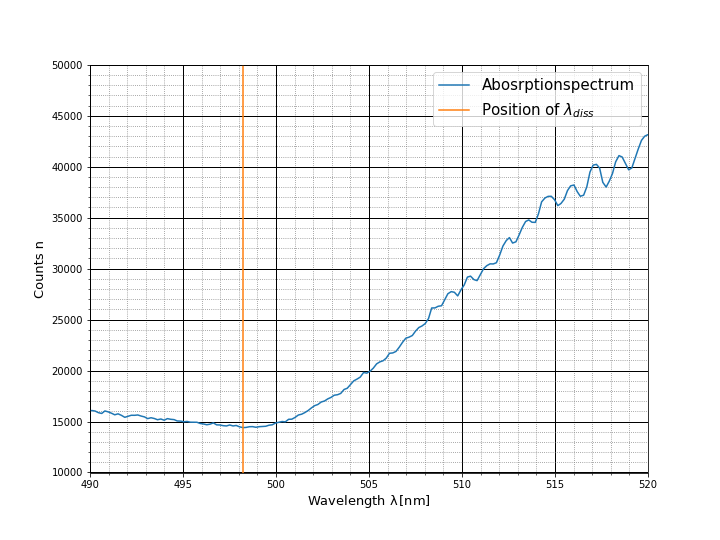
\includegraphics[scale=0.5]{Bild/AS_4.png}
	\centering
	\caption[Segment of the Absorption Spectrum]{\small Segment of the absorption spectrum, which is used to calculate the to find the wavelength $\lambda_{diss}$ which is marked in orange.}
	\label{figAS4}
\end{figure}
\subsubsection{The Morse Potential}
Last but not least the Morse potential shall depicted. For this we use equation \ref{eqMorse}. The needed constants $a$ and $R_e$ can be calculated with:
\begin{equation}
	a=\sqrt{\frac{\omega_ex_e4\pi c\mu}{\hbar}}
\end{equation}
\begin{equation}
	R_e=\sqrt{\frac{\hbar}{4\pi c\mu B_e}}
\end{equation}
With the constants:
$$c = 299792485\,\frac{\text{m}}{\text{s}}$$
$$\mu = 1.05327\times 10^{-25}\,\text{kg}$$
$$Be = 2.897,0.007\,\text{m}^{-1}$$
$$\hbar = 1.054571817\times 10^{-34}\,\text{J}$$
The equation for the Morse Potential is:
$$E_{Morse}=(4300\pm400\,)\text{cm}^{-1}\left(1-e^{-(1.98\pm0.06)\times10^{9}\,\text{m}^{-1}(R-(3.029\pm0.004)\times 10^{-10}\,\text{m})}\right)^2$$
This equation is plotted in figure \ref{figMorse}.
\begin{figure}[ht]
	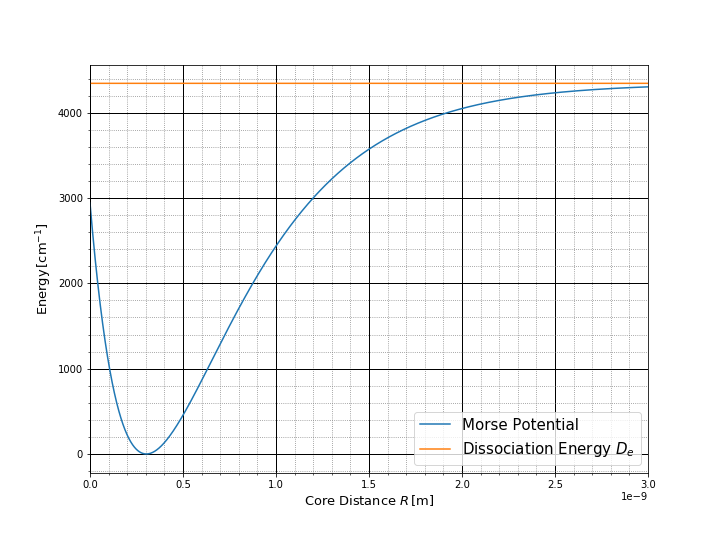
\includegraphics[scale=0.5]{Bild/Morse.png}
	\centering
	\caption[Calculated Morse Potential]{\small Morse potential with calculated values. In blue the Morse potential and in orange the dissociation energy which the Morse potential approaches for $R\rightarrow\infty$.}
	\label{figMorse}
\end{figure}
\subsection{Emission Spectrum}
\subsubsection{Calibration of the Monochromator}
For the calibration of the Monochromator we measured the spectrum of mercury vapour lamp. For the calibration only the data \verb|Eichung2.csv| was used since the first one distorted during the measurement.\par
First of all the $y$ values of the data were plotted against the wavelength which was calculated with the help of the starting position, end position and step width which were noted for each measurement. The plot can be seen in figure \ref{figEichung}.
On it four different peaks are visible. Each peak was fitted with a Gaussian normal distribution of the form \ref{eqGaus}.
\begin{equation}
f(x) = A \frac{1}{\sqrt{2\pi \sigma^2}} 	\exp\left(-\frac{1}{2}\frac{(x-x_c)^2}{\sigma^2}\right)+y_c
\label{eqGaus}
\end{equation}
Those fits are visible in figure \ref{figEichung} in red. The parameter $x_c$ gives the position of the peak and are noted together with the literature value in table \ref{ESWerte}. This way is used for all the future data of the monochromator as well.
\begin{table}[ht]
	\begin{Dtabular}[1.1]{|c|c|c|c|}
		\hline
		Name&Literature Value $\lambda\,$nm&Measured Values $\lambda$\,nm&$\Delta \lambda \,$nm\\
		\hline
		h-line&$404.66$&$404.88 \pm 0.05$&$0.22\pm 0.05$\\
		\hline
		g-line&$435.85$&$435.99 \pm 0.05$&$0.14\pm 0.05$\\
		\hline
		e-line&$546.07$&$546.46 \pm 0.05$&$0.39\pm 0.05$\\
		\hline
		double line $1$&$576.96$&$578.35 \pm 0.04$&$1.39\pm 0.04$\\
		\hline
		double line $2$&$579.07$&$578.35 \pm 0.04$&$-0.72\pm 0.04$\\
		\hline
	\end{Dtabular} 
	\centering
	\caption[Values of the Calibration Measurement]{Values of the fitted peaks as well as the literature values. There are also the differences between literature and measured value which shows a definite systematic error.}
	\label{ESWerte}
\end{table}
The since the resolution wasn't high enough, the double peak couldn't be split up. That's why these two measurements weren't used for the calibration. By taking the difference between the literature value and the measured ones and taking the mean of them we get the value by which all our measured values will be shifted. The error is calculated using the following equation:
\begin{equation}
	\sigma_{\Delta \lambda}=\lambda_{\text{Measured}} - \lambda_{\text{Literatur}}
\end{equation}
With that we get a systematic shift which will be subtracted from all further values. $$\Delta \lambda=(0.252\pm 0.028\,\text{nm})$$
\begin{figure}[ht]
	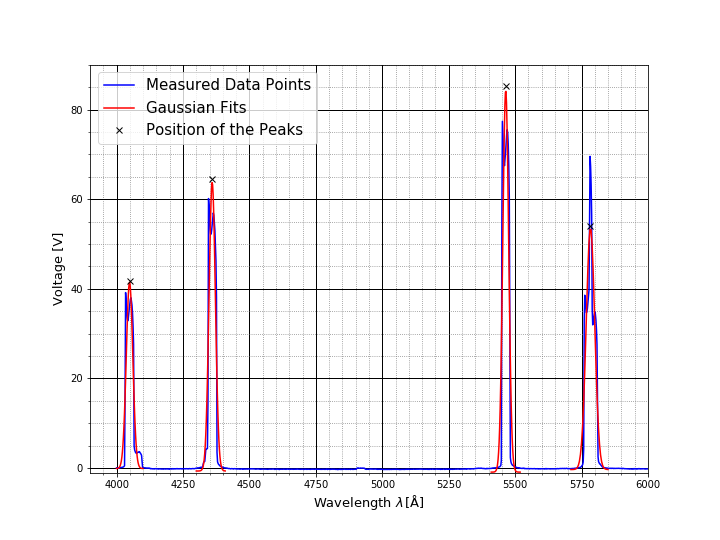
\includegraphics[scale=0.5]{Bild/QS.png}
	\centering
	\caption[Calibration with Mercury Vapour Lamp]{Peaks of the Calibration measurement with a mercury vapour lamp. In blue the measured data and in red the four Gaussian fits to the peaks.}
	\label{figEichung}
\end{figure}
\subsubsection{Laser Peak}
Next the laser peak should be depicted, for this the file \verb|Laserpeak.csv| was used and can be found in figure \ref{figLaser}.\par
Looking at data we see more like a laser plateau from $6317.5\text{\AA}$ to $6345.5\text{\AA}$. Because  of this the exact position couldn't be calculated but it still gives an indication in which area the peak is since the real peak will be somewhere in the area of the plateau. Since the plateau has a little drop after $6333.5\,\text{AA}$ we can decrease the area to an interval of $6317.5\text{\AA}$ to $6333.5\text{\AA}$. The Laser emits a light with a wavelength of $6330\,\text{\AA}$ which is in our designated area. 
\begin{figure}[ht]
	\includegraphics[scale=0.5]{Bild/Lpeak.png}
	\centering
	\caption[Laser Peak]{Measurement of the Laser Peak from $6300\,$\AA to $6370$\,\AA}
	\label{figLaser}
\end{figure}
\newpage
\subsubsection{$I_2$ Emission Spectrum}
In the last part of the experiment we measured the area of $6400\,\text{\AA}$ to $8000\,\text{\AA}$. This area was measured four times. Only the third measurement shows the later peaks clearly. The files \verb|emissionsspektrum1.csv|, \verb|emissionsspektrum2.csv| and \verb|emissionsspektrum4.csv| are depicted in the appendix. Used for the analysis only the file \verb|emissionsspektrum3.csv| was used which can be seen in figure \ref{figEMISSION}.
\begin{figure}[ht]
	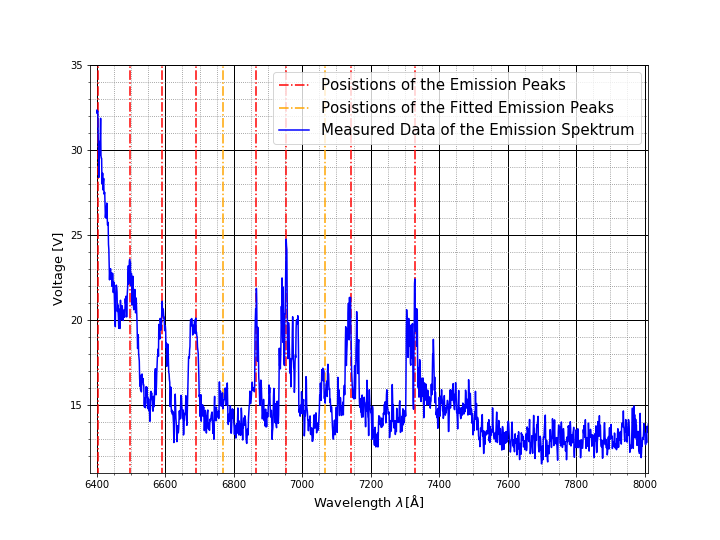
\includegraphics[scale=0.5]{Bild/E3_1.png}
	\centering
	\caption[Emission Spectrum with the found Peaks]{\small Emission Spectrum with the found Peaks. In orange the two smaller peaks calculated with Gaussian fits and in red the peaks found with PeakUtils.}
	\label{figEMISSION}
\end{figure}
To find the peaks we estimated the high peaks with the help of \verb|PeakUtils|\cite{Peak} by setting a high threshold value. The peaks which were found that way are marked in the figure \ref{figEMISSION} with red lines. Since there were two smaller Peaks in between which are clearly set apart from the background those two had to be fitted. In figure \ref{figGausEm}  those two were fitted with \verb|curve_fit| using equation \ref{eqGaus}. The position $x_c$ of the peak is marked in orange in figure \ref{figEMISSION}. As errors we estimated an error of $3\,\text{AA}$ for the ones calculated with \verb|PeakUtils|. For the ones fitted we used the error given by \verb|curve_fit|.\par
There is also a possible peak at around $7250\,\text{\AA}$ since there is a huge gab between the peaks besides. This one is very likely hidden in the noise. The $10$ found values which were measured, are in table \ref{LASTVALUE}. \par
To find out which transition we are looking at we calculate the energy of the wavelength using equation \ref{eqEnergie}, which can be found in said table as well. With the help of these values the correct transitions can be found by using the table \ref{TableSTAATSEXAMEN} which is also in the manual\cite{Anleitung}. The comparison indicates our measured transition are $\nu'=6 \rightarrow \nu''$ transitions by starting with $\nu''=4$ at the left to $\nu''=14$ at the right. Since there is a transition $\nu''=13$ we didn't found its likely that this one is the peak at $7250\,\text{\AA}$ which isn't visible. This idea is reinforced by the fact that the energy value given in table \ref{TableSTAATSEXAMEN} for the transition $\nu''=13$ is fitting with the position of the missing peak.
\begin{table}[ht]
	\begin{Dtabular}[1.1]{|c|c|c|c|c|}
		\hline
		Transition $\nu''$&Wavelength $\lambda$\,[\AA]&Energy $G(\nu'')\,[\text{cm}^-1]$&Literature Value  $G(\nu'')\,[\text{cm}^-1]$&Comparison [$\sigma$]\\
		\hline
		$4$&$ 6402.0 \pm 3.0 $&$ 15632 \pm 7 $&$15602.5068$&$3.23$\\
		$5$&$ 6496.0 \pm 3.0 $&$ 15406 \pm 7 $&$15394.0768$&$0.84$\\
		$6$&$ 6591.0 \pm 3.0 $&$ 15184 \pm 7 $&$15186.8608$&$ 1.28$\\
		$7$&$ 6689.0 \pm 3.0 $&$ 14961 \pm 7 $&$14980.8588$&$3.76$\\
		$8$&$ 6768.5 \pm 1.3 $&$ 14785.3 \pm 3.1 $&$14776.0708$&$ 1.26$\\
		$9$&$ 6866.0 \pm 3.0 $&$ 14575 \pm 6 $&$14572.4968$&$0.41$\\
		$10$&$ 6953.0 \pm 3.0 $&$ 14393 \pm 6 $&$14370.1368$&$2.78$\\
	    $11$&$ 7066.6 \pm 0.8 $&$ 14161.1 \pm 2.0 $&$14168.9908$&$7.41$\\
		$12$&$ 7141.0 \pm 3.0 $&$ 14014 \pm 6 $&$13969.0588$&$6.68$\\
		$13$&$7250$&$13793$&$13770.3408$&-\\                
		$14$&$ 7329.0 \pm 3.0 $&$ 13654 \pm 6 $&$13572.8368$&$13.59$\\
		\hline
	\end{Dtabular}
	\centering
	\caption[Values of the Emission Spectrum]{Values of the Emission Spectrum. With the likely transition and literature values. In the last column is the comparison between the calculated energy and the likely literature values. The values are compared using equation \ref{vgl} and are in the units of the standard deviation.}
	\label{LASTVALUE}
\end{table}